\section{Dataset and Annotation Audit}
\subsection{Evidence and scope}
The dataset description combines two evidence sources. A local audit dated 7 October 2026 reports full image and mask decoding, polygon comparisons, and duplicate screening~\cite{localaudit}. For this manuscript, metadata, file presence, annotation references, and the actual annotation-builder output were rechecked on 30 October 2026~\cite{snapshot}. This structural recheck did not repeat the pixel-level audit, duplicate search, or model inference. Historical audit findings are identified accordingly.

\begin{table}[t]
\centering\small
\caption{Local dataset releases. Disease counts refer to underlying labels; v6 metadata exposes only 114 IDs because of a soybean-rust labeling error. Coverage statistics are calculated from metadata.}
\label{tab:versions}
\begin{tabular}{lrr}\toprule
Property & v6 & v7\\\midrule
Image--mask pairs & 11,458 & 7,774\\
Training images & 7,916 & 5,367\\
Validation images & 1,247 & 846\\
Test images & 2,295 & 1,561\\
Host plants & 34 & 34\\
Disease categories & 115 & 115\\
Mean coverage (\%) & 21.4 & 21.4\\
Median coverage (\%) & 13.7 & 13.9\\\bottomrule
\end{tabular}
\end{table}

\subsection{Release selection and label representation}
The current script defaults to v7. Its 7,774 images are partitioned into 5,367 training, 846 validation, and 1,561 test samples (Table~\ref{tab:versions}). The previous audit reports that v7 retains a byte-identical subset of 7,774 v6 images and masks, with no split changes. Thus v6 and v7 must not be treated as independent datasets or used as separate training and test domains.

Each image has a same-stem PNG semantic mask and an associated metadata row. The mask value 0 denotes background, while nonzero values represent disease IDs offset by one. Each image has one labeled disease, potentially occupying multiple disconnected regions. The semantic mask therefore does not, by itself, define lesion instance identities. COCO polygon annotations supply the instance-style supervision consumed by the current training script.

Metadata provides disease names, plant names, class indices, split membership, and mask coverage. The v7 CSV requires UTF-8 BOM handling. The raw COCO files have empty category lists, so class names cannot be recovered from those lists alone. The training builder reconstructs categories from metadata. Its use of image-level metadata also overrides conflicting annotation category IDs; this is a labeling policy, not an independent confirmation of biological correctness.

\begin{figure*}[t]
\centering
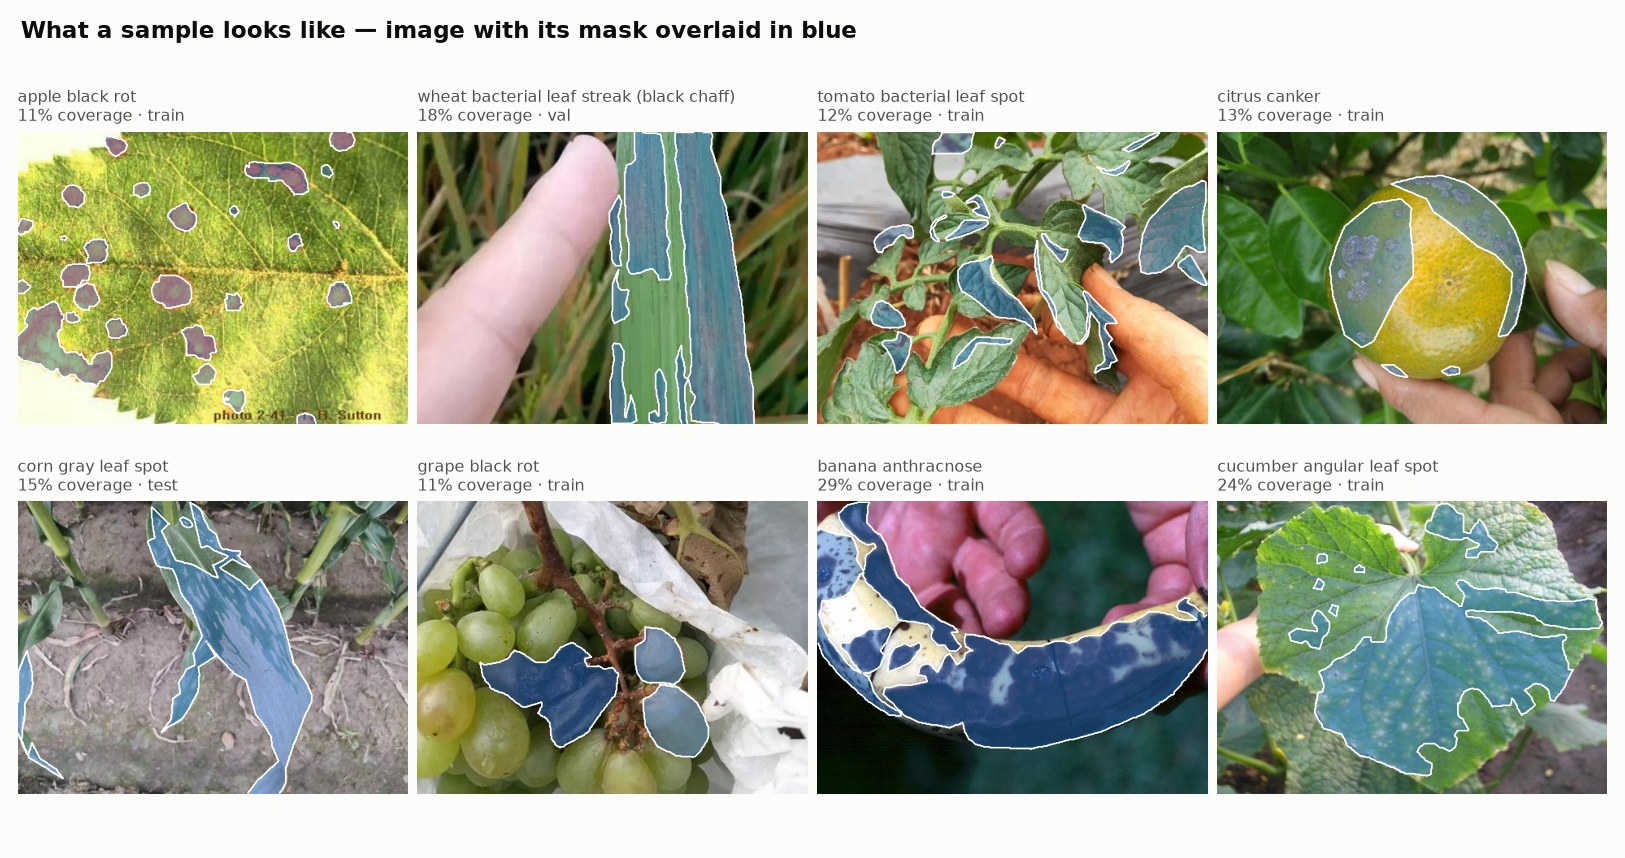
\includegraphics[width=\textwidth]{figures/dataset_samples.jpg}
\caption{PlantSeg examples from the existing local audit, with PNG ground-truth masks overlaid in blue. They illustrate fragmented spots, elongated symptoms, and extensive diseased regions. These are annotation examples, not model predictions. Source: local dataset audit~\cite{localaudit}.}
\label{fig:samples}
\end{figure*}

\subsection{Class and foreground imbalance}
The prior audit reports a long-tailed distribution: v7 class sizes range from 3 to 323 images, and 26 disease categories have fewer than 20 training images. Coffee black rot has no test image, while peach rust has no validation image. A class macro-average must therefore state the eligible class set and cannot silently assume support for every class in every partition.

Mean foreground coverage is approximately 21.4\%, with median coverage 13.9\%. The earlier pixel audit estimates that diseased pixels occupy 19.4\% of all v7 pixels when weighted by image size. Image-averaged coverage and pixel-weighted coverage are different statistics. Small regions can consequently contribute little to global pixel scores even when clinically or visually salient. Figure~\ref{fig:samples} illustrates the variety of annotation extent, including whole-region labels and individual spots.

\subsection{Raw and effective polygon supervision}
The structural recheck confirms that v7 retains 77,394 raw annotation records, of which 21,580 refer to image IDs absent from their split. The surviving records total 55,814. The project builder filters these orphan records, rejects polygons with invalid coordinate counts and boxes smaller than one pixel, normalizes numeric fields, and drops images with no remaining annotation.

\begin{table}[t]
\centering\small
\caption{Rechecked v7 annotation counts. ``Effective images'' are produced by the current builder before stochastic training transforms.}
\label{tab:effective}
\begin{tabular}{lrrr}\toprule
 & Train & Val. & Test\\\midrule
Raw images & 5,367 & 846 & 1,561\\
Raw polygons & 52,898 & 8,927 & 15,569\\
Orphan polygons & 14,647 & 2,467 & 4,466\\
Retained polygons & 38,251 & 6,460 & 11,103\\
Effective images & 5,367 & 846 & 1,560\\\bottomrule
\end{tabular}
\end{table}

The single excluded test image has a PNG mask but no polygon annotation. Therefore the script's effective polygon test set has 1,560 images, whereas a PNG-mask evaluation can retain all 1,561. Both the reference type and evaluated sample count must accompany any final score.

\subsection{Quality issues beyond structural filtering}
The earlier audit reports 180 v7 images whose polygons belong to another image, including 163 training samples. Structural filtering does not repair these shapes. The same audit identifies 107 validation and 183 test images with an exact or near duplicate in training. These are screened duplicate candidates based on image hashing and local review; the full duplicate analysis was not rerun for this paper.

Additional reported issues include conflicting disease labels and nine images with EXIF orientation flags. The inspected image loader converts opened images to RGB without an explicit EXIF transpose at that location. Orientation alignment must therefore be checked before a final experiment. The present training path also does not remove flagged duplicates or regenerate instances from PNG masks. These remain required preparation choices for the quality-controlled study described in Section~\ref{sec:protocol}.
